\date{September 2020}

\documentclass[conference]{IEEEtran}
\usepackage{xcolor}
\usepackage[utf8]{inputenc}
\usepackage{graphicx}
\usepackage{fixltx2e}
\usepackage{upgreek}
\usepackage{amsmath}
\usepackage{amsfonts}
\usepackage{amssymb}
\usepackage{mathtools}
\usepackage{float}
\usepackage{multicol}
\usepackage{blkarray}
\usepackage{tabularx}
\usepackage{gensymb}
\usepackage{subcaption}
\usepackage[font=small,labelfont=bf]{caption}
\usepackage{pgfgantt} % Gantt chart package
\PassOptionsToPackage{hyphens}{url}\usepackage{hyperref} % line breaks for links with the \url command
\usepackage{rotating} % landscape figures
\usepackage{comment} % multiline comments
\usepackage{listings}

\lstset{
  aboveskip=3mm,
  belowskip=3mm,
  showstringspaces=false,
  columns=flexible,
  basicstyle={\small\ttfamily},
  numbers=none,
  breaklines=true,
  breakatwhitespace=true,
  tabsize=3
}

\usepackage[style=ieee]{biblatex}
\addbibresource{references.bib}

\title{Backprogagation}

\author{\IEEEauthorblockN{JingYang Zeng, David Pomerenke} 
\textit{Advanced Concepts of Machine Learning (Kurt Driessens) 2020} \\
\IEEEauthorblockA{\textit{Department of Data Science and Knowledge Engineering, Maastricht University}
}} 


% comment possibilities for all authors
\usepackage{color}
\usepackage{xcolor}
\newcommand{\todo}[1]{\textcolor{violet}{TODO #1}} % dp is already defined

\begin{document}

\maketitle

\thispagestyle{plain} % page numbers!
\pagestyle{plain} % page numbers!

\begin{abstract}
    We implement the backpropagation algorithm for artificial neural networks, and applied it to a simple synthetic classification problem. Our implementation achieves an optimal encoding with a modest training time of only 50 epochs.
\end{abstract}

% \tableofcontents


\section{Implementation}

We implement the neural network in Python, making use of the \textit{numpy} library\footnote{\url{https://numpy.org}} for fast vector mathematics. We mainly follow the implementation by Ng\cite{ng_sparse_2011}, enriching it with additional alternative activation functions.

\subsection{Documentation}

The core functionality is found in \textit{src/neural\_network.py}.

The training data (both input and output) is of the form of vectors of a fixed size $n_l$, where exactly one value is set to $1$, and all other values are set to $0$. These data are generated by the function \textit{generate\_dataset}, which takes the size as an argument and returns the list of all possible data with this size.

We store the weights $W_l$ and $b_l$ in a dictionary called \textit{parameters}. Initial random values for these parameters are created with \textit{initialize\_parameters}, optionally taking a seed number as an argument.

Once the test data are generated and the parameters are initialized, a network can be trained with \textit{train\_model}. This takes the input data, output data, an array indicating the shape of the neural network, and the two hyperparameters: learning rate and iteration count. This function can create networks of any size and shape, so it is more general than required for this assignment; but we will make some use of this advantage in our analysis of the weights.

The functionality related to the activation functions is provided in \textit{src/kernel.py}. We provide implementations of multiple activation functions: 

The sigmoid function $f(x) = \frac{1}{1+e^{-x}}$, the hyperbolic tangent $f(x) = \frac{e^x-e^{-x}}{e^x-e^{-x}}$, the softmax function
$f(x) = \frac{e^x}{\sum_{i=1}^n e^{x_i}}$, the rectifier $f(x) = \max(0,x)$, and the linear function $f(x) = x$, and their respective derivatives.

\textit{forward\_propagation} performs a forward propagation from the activations of one level of units, returning the activations of the next level, taking the activation function to be used as an argument. \textit{backward\_propagation} does the same for the backpropagation of the errors. We do not use a regularization term for the calculation of the errors, thus there is no weight decay parameter.

\textit{tests/test.py} contains the code for the analysis further described in this document.

\subsection{Instructions}

We use \textit{Poetry}\footnote{\url{https://python-poetry.org/docs}}\footnote{\url{https://python-poetry.org/docs/basic-usage}} as a deterministic project dependency manager. The code can be executed as follows:

\begin{lstlisting}
    poetry install
    poetry run python tests/test.py
\end{lstlisting}

Alternatively, we have provided a \textit{requirements.txt} for usage with \textit{pip}. Since--unlike \textit{poetry}--pip installs dependencies globally, this will require the manual setup of a virtual environment.

\section{Learning performance}

We encountered the following problem: When we implement the neural network, at first we mistakenly used a sigmoid function for our last hidden layer; with that configuration, even after iterating 10000 times there was still an overall cost of 0.77, and we could only achieve an accuracy up to 0.625.

Then we realized our task is a multiple classification rather than binary classification; the sigmoid function would like a Bernoulli distribution, each value in result is independent of all other values, but the expected results are 8 distinguished predictions and should only have a “1” in each result. Therefore, we used \textit{softmax} and cross-entropy loss, which works for multiple classification, as an activation function for our last layer, which dramatically improved the expected result.

The results of testing our implementation with multiple learning rates and iteration counts are presented in Figure \ref{fig:performance}. Smaller and larger values than displayed have been tried out and have been discarded.

\begin{figure}
    \centering
    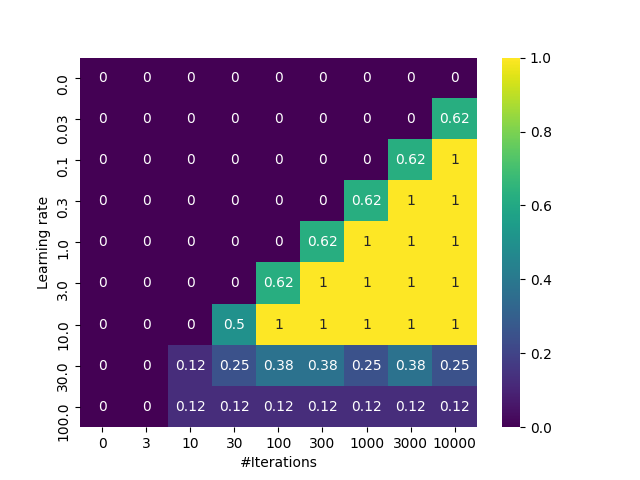
\includegraphics[width=10cm]{learning_performance.png}
    \caption{Accuracy given the learning rate and the number of iterations.}
    \label{fig:performance}
\end{figure}

A short number of iterations is preferable (given the same accuracy). The best set of hyperparameters is thus a learning rate of $\approx10$ and an iteration count of $\approx100$.

The cost given the number of iterations is displayed for 2 selected learning rates: For $10$ (see Figure \ref{fig:cost1}), which is near the optimal learning rate (which we know from Figure \ref{fig:performance}), and for an substantially lower learning rate of $0.1$ (see \ref{fig:cost2}). We can see that the learning rate has a dramatic impact on the number of learning iterations that is required for good predictions.

\begin{figure}
    \centering
    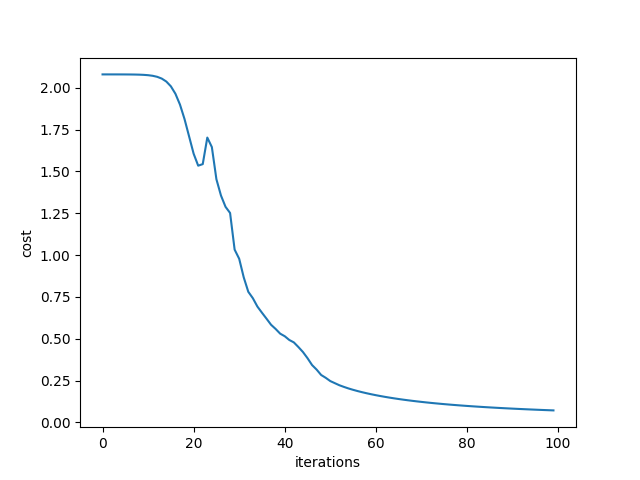
\includegraphics[width=9cm]{cost1.png}
    \caption{Cost given the number of iterations for a fixed learning rate of $10$. This is near the optimal learning rate.}
    \label{fig:cost1}
\end{figure}

\begin{figure}
    \centering
    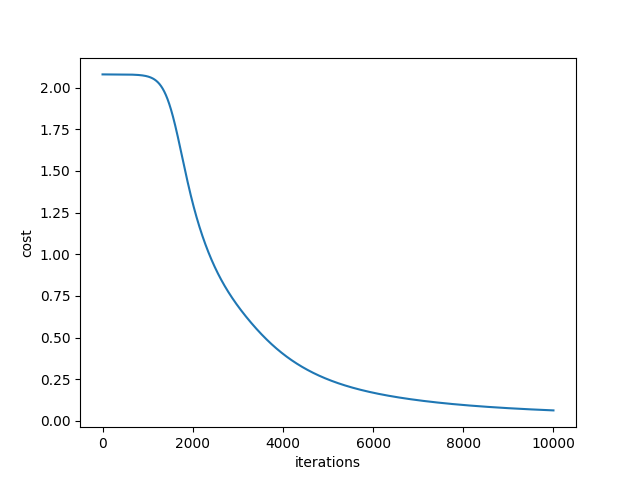
\includegraphics[width=9cm]{cost2.png}
    \caption{For comparison: Cost given the number of iterations for a fixed learning rate of $0.1$.}
    \label{fig:cost2}
\end{figure}

\section{Interpretation}

There is only one layer of hidden units. The activations of these units for input data where unit $i$ takes the value $1$ and the rest takes the value $0$ are thus identical to the weights and biases coming in from unit $i$. 

\begin{figure}
    \centering
    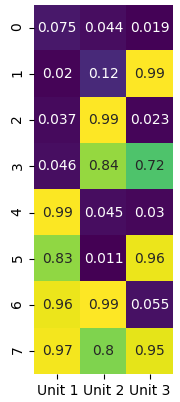
\includegraphics[height=7cm]{hidden1.png}
    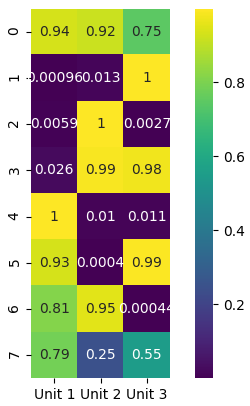
\includegraphics[height=7cm]{hidden2.png}
    \caption{Visualization of the weights and biases (normalized by a sigmoid function) for the 8 input data. Connections between input units and hidden units (left) and between hidden units and output units (transposed, right). The former are identical to the activations of the hidden layer for the respective data. The order of the rows has been adjusted manually.}
    \label{fig:hidden}
\end{figure}

We observe that the weights encode the 8 categories in a binary fashion -- see Figure \ref{fig:hidden}, and compare with Figure \ref{fig:truthtable}! This is the most efficient encoding possible, since $8=2^3$ categories have to be compressed into $3$ units. It is positively surprising that the network so intellegintly finds this representation.

\begin{figure}
    \centering
    \begin{tabular}{l|lll}
    0 & 0 & 0 & 0 \\
    1 & 0 & 0 & 1 \\
    2 & 0 & 1 & 0 \\
    3 & 0 & 1 & 1 \\
    4 & 1 & 0 & 0 \\
    5 & 1 & 0 & 1 \\
    6 & 1 & 1 & 0 \\
    7 & 1 & 1 & 1 \\
    \end{tabular}
    \caption{Binary encodings of the first eight numbers, for comparison.}
    \label{fig:truthtable}
\end{figure}

We verify our hypothesis about the efficient encoding by training a network of shape \textit{16--4--16} with 16 different vectors in analogy to the 8-vector training set used before. The results can be seen in Figure \ref{fig:hidden16}: Indeed, we can again find the truth-table-like structure in the trained weights.

\begin{figure}
    \centering
    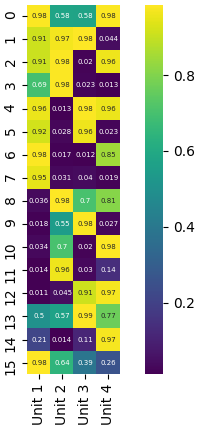
\includegraphics[height=12cm]{hidden16.png}
    \caption{Visualization of the weights and biases (normalized by a sigmoid function) for 16 input data. Connections between input units and hidden units. The rows have been ordered manually to match the truth-table for 4 bits. We use the same hyperparameters as above (a learning rate of $10$), but extend the number of iterations from $100$ to $200$.}
    \label{fig:hidden16}
\end{figure}


\printbibliography

\newpage


\end{document}